\documentclass[11pt,a4paper]{article}
\usepackage[T1]{fontenc}
\usepackage[utf8]{inputenc}
\usepackage{lmodern}
\usepackage[a4paper,left=2.2cm,right=2.2cm,top=2.1cm,bottom=2.1cm,headheight=15pt,headsep=14pt]{geometry}
\usepackage{graphicx,xcolor,booktabs,tabularx,array}
\usepackage{microtype,fancyhdr,titlesec,enumitem,float,caption,listings,xurl}
\usepackage[unicode,colorlinks=true,linkcolor=teal,urlcolor=teal]{hyperref}
\definecolor{ink}{HTML}{183B50}
\definecolor{teal}{HTML}{14675F}
\definecolor{paper}{HTML}{F1F5F7}
\definecolor{line}{HTML}{B8C9D1}
\hypersetup{pdftitle={Laporan Praktikum Web Service Lab 08 - API Gateway},
  pdfauthor={Bambang Herlambang},pdfsubject={Tugas individu - 5803024019}}
\graphicspath{{images/}}
\pagestyle{fancy}
\fancyhf{}
\fancyhead[L]{\small\color{ink}Praktikum Web Service / Lab 08}
\fancyhead[R]{\small\color{ink}Bambang Herlambang}
\fancyfoot[L]{\small\color{ink}5803024019 \enspace | \enspace Tugas individu}
\fancyfoot[R]{\small\color{ink}Halaman \thepage}
\renewcommand{\headrulewidth}{0.4pt}
\renewcommand{\footrulewidth}{0pt}
\titleformat{\section}{\large\bfseries\color{ink}}{\thesection.}{0.5em}{}
\titleformat{\subsection}{\normalsize\bfseries\color{ink}}{\thesubsection}{0.5em}{}
\titlespacing*{\section}{0pt}{8pt}{7pt}
\titlespacing*{\subsection}{0pt}{8pt}{4pt}
\setlength{\parindent}{0pt}
\setlength{\parskip}{5pt}
\setlength{\intextsep}{6pt}
\setlength{\textfloatsep}{8pt}
\setlength{\emergencystretch}{2em}
\renewcommand{\arraystretch}{1.18}
\renewcommand{\figurename}{Gambar}
\renewcommand{\tablename}{Tabel}
\captionsetup{font=small,labelfont=bf,labelsep=period,skip=5pt,justification=raggedright,singlelinecheck=false}
\setlist[itemize]{leftmargin=1.3em,itemsep=2pt,topsep=3pt}
\newcolumntype{L}[1]{>{\raggedright\arraybackslash}p{#1}}
\newcolumntype{Y}{>{\raggedright\arraybackslash}X}
\newcommand{\code}[1]{\texttt{\detokenize{#1}}}
\lstset{basicstyle=\small\ttfamily,backgroundcolor=\color{paper},
  frame=single,rulecolor=\color{line},breaklines=true,columns=fullflexible,
  keepspaces=true,showstringspaces=false,aboveskip=6pt,belowskip=6pt,
  xleftmargin=7pt,xrightmargin=7pt,framexleftmargin=5pt,framexrightmargin=5pt}
\newcommand{\postmanshot}[1]{\includegraphics[width=.90\linewidth,trim=160bp 12bp 0bp 56bp,clip]{#1}}
\begin{document}
{\color{teal}\small LAPORAN PRAKTIKUM WEB SERVICE SESI 08}\par
{\color{ink}\LARGE\bfseries API Gateway Sederhana}\par
{\large Node.js dan Express}\par
\vspace{4pt}
\begin{tabularx}{\linewidth}{@{}L{2.0cm}Y@{}}
Nama & Bambang Herlambang\\
NIM & 5803024019\\
Pengerjaan & Individu\\
Tanggal & 21 Oktober 2026\\
Repository & \href{https://github.com/academicbambang/prakwebservice-lab08-api-gateway}{academicbambang/prakwebservice-lab08-api-gateway}\\
\end{tabularx}
\vspace{5pt}
{\color{teal}\hrule height 1.1pt}
\vspace{6pt}

\section{Tujuan dan ruang lingkup}
Praktikum ini membangun satu pintu masuk untuk dua service demo: Catalog Service
dan Order Service. Gateway meneruskan request berdasarkan path, membatasi
request menjadi 20 per 10 detik per alamat IP, serta memeriksa API key pada
jalur pesanan. Implementasi mengikuti Opsi A Lab 08 dengan Node.js, Express,
\code{http-proxy-middleware}, dan \code{express-rate-limit}.

Hasil yang ditunjukkan meliputi akses kedua service melalui port 8080, penolakan
akses tanpa key, dan perubahan respons menjadi \code{429} ketika kuota
terlampaui. Tugas dikerjakan secara individu; kedua service dipakai sebagai
konteks demonstrasi gateway. Materi Web Service menjadi acuan keamanan API key,
sedangkan materi Software Testing menjadi acuan pengujian batas dan skenario
negatif.

\begin{figure}[H]
\centering
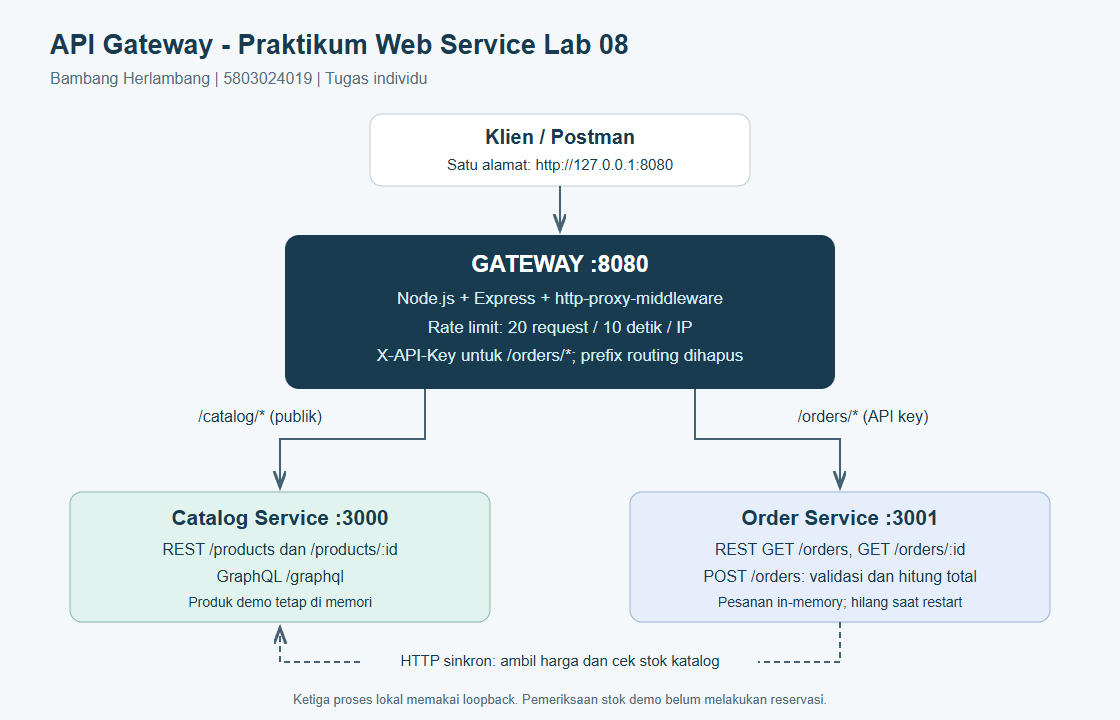
\includegraphics[width=.94\linewidth]{arsitektur.png}
\caption{Arsitektur implementasi lokal. Order Service mengambil harga dan
memeriksa stok melalui panggilan HTTP sinkron ke Catalog Service.}
\label{fig:arsitektur}
\end{figure}

\clearpage
\section{Arsitektur dan implementasi}
\subsection{Routing dua service}
Klien cukup menggunakan \code{http://127.0.0.1:8080}. Prefix \code{/catalog}
atau \code{/orders} dihapus sebelum request diteruskan ke port 3000 atau 3001.
Query string dan body tetap diteruskan.

\begin{table}[H]
\centering\small
\begin{tabularx}{\linewidth}{@{}L{1.35cm}Y Y@{}}
\toprule
Method & Path pada gateway & Path pada service\\
\midrule
GET & \path{/catalog/products} & Catalog \path{/products}\\
GET & \path{/catalog/products/:id} & Catalog \path{/products/:id}\\
POST & \path{/catalog/graphql} & Catalog \path{/graphql}\\
GET & \path{/orders/orders} & Order \path{/orders}\\
GET & \path{/orders/orders/:id} & Order \path{/orders/:id}\\
POST & \path{/orders/orders} & Order \path{/orders}\\
\bottomrule
\end{tabularx}
\caption{Pemetaan endpoint melalui gateway.}
\end{table}

Path \code{/orders/orders} disengaja: bagian pertama merupakan namespace
gateway dan bagian kedua merupakan resource pada Order Service. Endpoint
\code{GET /health} tersedia pada ketiga proses.

\subsection{Rate limiting, API key, dan penerusan request}
Middleware rate limit dipasang sebelum routing. Semua endpoint gateway,
termasuk health check, respons \code{401}, dan route tidak dikenal, berbagi
kuota untuk IP yang sama. Request ke-21 dalam window yang sama mendapat
\code{429 Too Many Requests}. Penghitung memakai memori satu proses.

Katalog bersifat publik, sedangkan jalur pesanan memerlukan header
\code{X-API-Key}. Key yang tidak ada atau tidak cocok ditolak dengan
\code{401 Unauthorized}. Pemeriksaan menggunakan digest SHA-256 dan
\code{timingSafeEqual}; digest server juga dapat diberikan melalui
\code{API_KEY_SHA256}. Key asli dihapus dari request yang diteruskan ke upstream.

Gateway tidak memasang \code{express.json()} sebelum proxy sehingga body
request tetap utuh. Parsing dilakukan pada service tujuan. Header
\code{Location} relatif dari upstream ditulis ulang dengan prefix gateway
agar tautan detail pesanan tetap melewati gateway. Upstream yang tidak
tersedia menghasilkan respons \code{502} yang terkendali.

\subsection{Konfigurasi dan data demo}
Konfigurasi gateway berada di \path{gateway/.env}; contoh tanpa secret tersedia
dalam \path{gateway/.env.example}. File \code{.env} diabaikan oleh Git.

\begin{table}[H]
\centering\small
\begin{tabularx}{\linewidth}{@{}L{4.8cm}Y@{}}
\toprule
Variabel & Pengaturan lokal / fungsi\\
\midrule
\code{HOST}, \code{PORT} & \code{127.0.0.1}, \code{8080}\\
\code{CATALOG_SERVICE_URL} & \code{http://127.0.0.1:3000}\\
\code{ORDER_SERVICE_URL} & \code{http://127.0.0.1:3001}\\
\code{API_KEY}, \code{API_KEY_SHA256} & Key acak lokal atau digest alternatif\\
\code{TRUST_PROXY} & \code{0} untuk koneksi lokal langsung\\
\code{CATALOG_PORT}, \code{ORDER_PORT} & Port backend \code{3000} dan \code{3001} pada stack\\
\bottomrule
\end{tabularx}
\caption{Konfigurasi utama. Port backend terpisah dari variabel \code{PORT}.}
\end{table}

Catalog Service menyediakan REST dan GraphQL. Order Service mengambil harga
produk dari katalog, memvalidasi kuantitas, serta menghitung total pesanan.
Data disimpan dalam memori; stok diperiksa tanpa reservasi atau pengurangan.

\clearpage
\section{Prosedur dan rancangan pengujian}
\subsection{Reproduksi lingkungan lokal}
Gunakan Node.js 22 atau lebih baru. Dari root repository, jalankan:
\begin{lstlisting}
npm install
npm run setup
npm start
\end{lstlisting}
Setup membuat key acak pada \path{gateway/.env}. Import collection dan
environment di \path{docs/postman} ke Postman, pilih environment lokal,
kemudian isi variabel \code{apiKey} dengan key asli untuk klien. Jangan
mengirim digest server sebagai key klien.

Untuk menjalankan proses secara terpisah, gunakan tiga terminal:
\begin{lstlisting}
node catalog-service/server.js
node order-service/server.js
node gateway/gateway.js
\end{lstlisting}
Perintah \code{node gateway.js} juga dapat dijalankan dari folder
\code{gateway} setelah kedua backend aktif.

\subsection{Strategi dan skenario}
Suite memakai \code{node:test}. Unit test memeriksa logika yang terisolasi,
integration test memeriksa perilaku HTTP, dan pengujian alur menyeluruh
menghubungkan gateway dengan kedua service nyata. Boundary Value Analysis
(BVA) diterapkan pada batas kuota 20/21 serta batas kuantitas pesanan;
skenario negatif diperiksa dengan assertion otomatis.

\begin{table}[H]
\centering\small
\begin{tabularx}{\linewidth}{@{}L{1.15cm}Y L{4.6cm}@{}}
\toprule
ID & Skenario & Hasil yang diharapkan\\
\midrule
GW-01 & Katalog melalui gateway & \code{200}, data katalog\\
GW-02 & Pesanan dengan key benar & \code{200}, data Order Service\\
GW-03 & Key tidak ada atau salah & \code{401}, akses ditolak\\
GW-04 & Penghapusan prefix dan query & Path serta query sesuai upstream\\
GW-05 & POST JSON GraphQL dan pesanan & Body utuh, respons selesai\\
GW-06 & Route tidak terdaftar & \code{404}\\
GW-07 & 30 request pada window bersih & 20 respons \code{200}, lalu 10 \code{429}\\
GW-08 & Window rate limit berakhir & Kuota kembali tersedia\\
GW-09 & Input pesanan tidak valid & \code{400}, pesanan tidak dibuat\\
GW-10 & Upstream tidak tersedia & \code{502}, request tidak menggantung\\
\bottomrule
\end{tabularx}
\caption{Skenario fungsional, batas, dan negatif.}
\end{table}

Jalankan \code{npm test} untuk suite otomatis. Untuk demonstrasi rate limit,
hentikan stack terlebih dahulu lalu jalankan \code{npm run test:rate-limit}.
Skrip membuat gateway baru di port 8080 dan mengirim 30 request berurutan.
Jika menguji server yang sudah aktif dengan \code{node gateway/test-rate-limit.js},
tunggu setidaknya 10 detik tanpa request sebelumnya dari IP yang sama.

\clearpage
\section{Bukti akses kedua service melalui gateway}
Kedua tangkapan layar menunjukkan port gateway yang sama, yaitu 8080.
Tampilan dipotong pada tata letak dokumen untuk memperbesar area request dan
respons; berkas gambar asli tetap tersedia dalam repository.

\begin{figure}[H]
\centering
\postmanshot{postman-catalog.png}
\caption{Postman: \code{GET /catalog/products?search=kopi} melalui gateway
menghasilkan \code{200} dan data produk sesuai pencarian.}
\label{fig:catalog}
\end{figure}

\begin{figure}[H]
\centering
\postmanshot{postman-orders.png}
\caption{Postman: \code{GET /orders/orders} dengan key benar menghasilkan
\code{200}, \code{service: order-service}, dan daftar \code{data: []}.
Nilai key tidak ditampilkan.}
\label{fig:orders}
\end{figure}

\clearpage
\section{Verifikasi autentikasi dan pengujian otomatis}
\begin{figure}[H]
\centering
\postmanshot{postman-unauthorized.png}
\caption{Postman: request pesanan tanpa header \code{X-API-Key} ditolak
gateway dengan \code{401 Unauthorized}.}
\label{fig:unauthorized}
\end{figure}

\subsection{Hasil suite otomatis}
Eksekusi \code{npm test} menghasilkan \textbf{35 test lulus dari 35 test},
tanpa kegagalan. Ringkasan berikut berasal dari log eksekusi
\path{docs/evidence/tests.txt}.
\begin{lstlisting}
1..35
# tests 35
# pass 35
# fail 0
# cancelled 0
# skipped 0
# todo 0
# duration_ms 2805.1146
\end{lstlisting}

Pengujian alur nyata memeriksa katalog dan GraphQL melalui gateway, penolakan
tanpa key, pembuatan pesanan \code{prod-001} sebanyak dua unit, total
Rp170.000 dari harga katalog, pengambilan detail melalui header
\code{Location}, serta daftar pesanan. Daftar kosong pada
Gambar~\ref{fig:orders} berasal dari proses demo yang baru dijalankan;
bukti pembuatan pesanan terdapat dalam suite otomatis.

Log memuat warning deprecation \code{DEP0060} terkait \code{util._extend}
pada dependency proxy. Warning tersebut tidak menggagalkan assertion;
hasil ini tidak dinyatakan sebagai eksekusi tanpa warning.

\clearpage
\section{Bukti rate limiting}
Demonstrasi memakai batas default \textbf{20 request per 10 detik per IP}.
Skrip mengirim 30 request ke
\code{http://127.0.0.1:8080/catalog/products} dengan kuota awal yang bersih.

\begin{figure}[H]
\centering
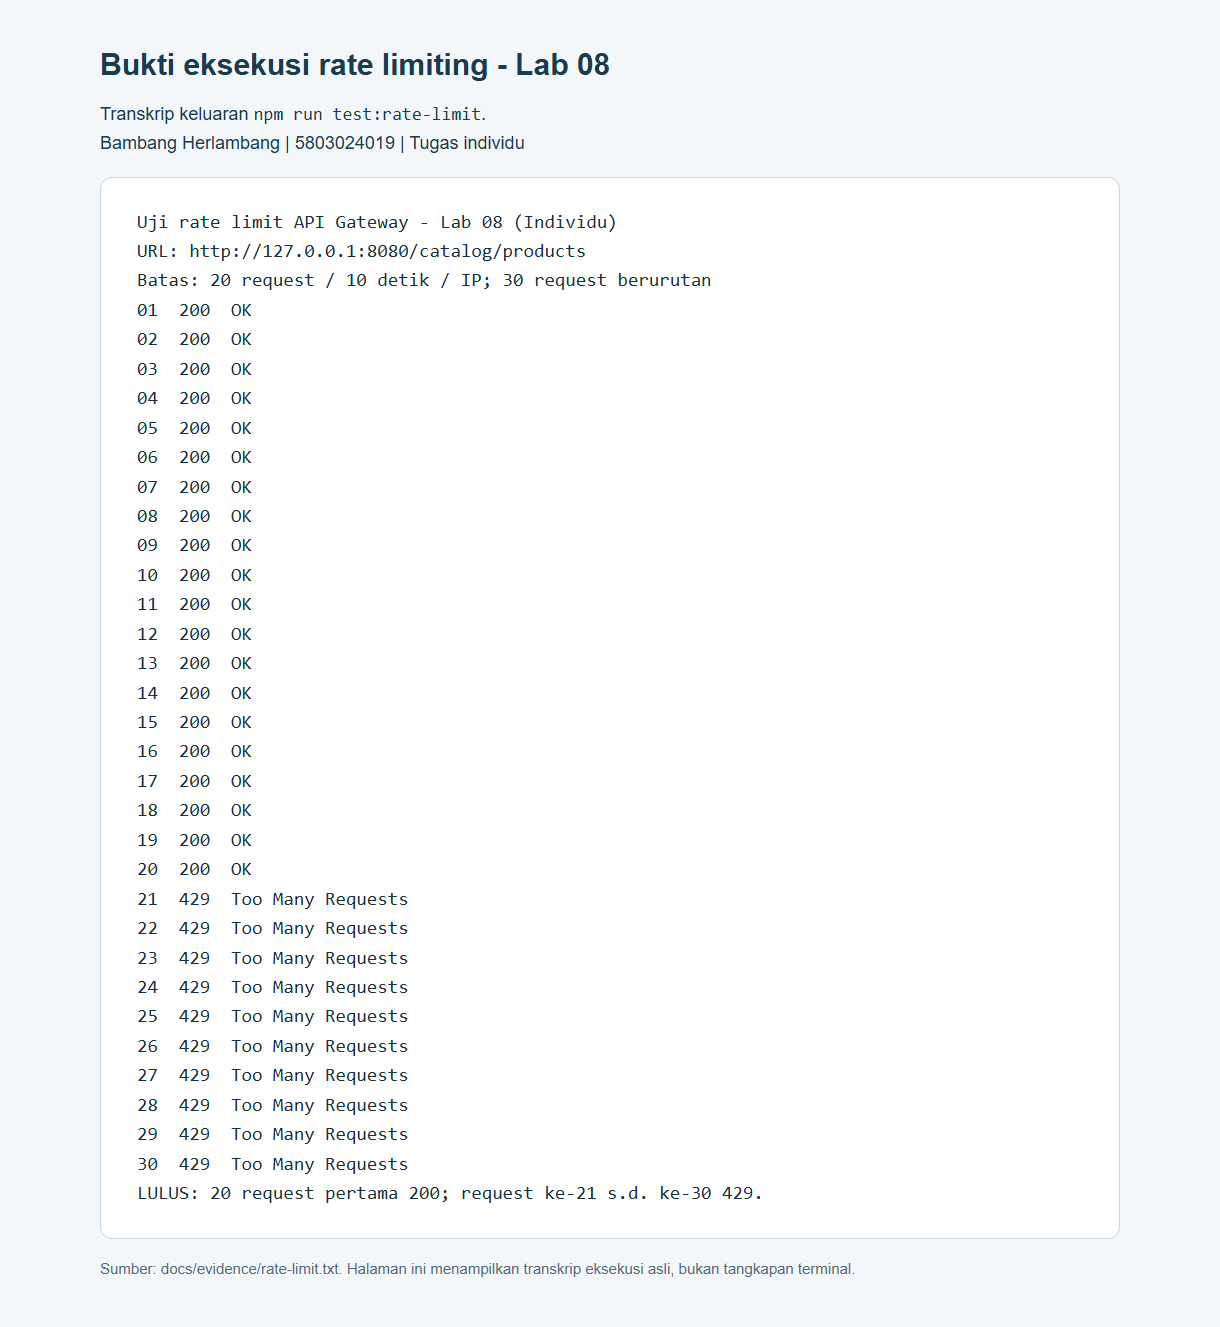
\includegraphics[width=\linewidth,height=.77\textheight,keepaspectratio]{rate-limit.png}
\caption{Tangkapan halaman transkrip keluaran
\code{npm run test:rate-limit}, bersumber dari log eksekusi asli
\texttt{docs/evidence/rate-limit.txt}; bukan tangkapan terminal langsung.}
\label{fig:rate}
\end{figure}

Request 1--20 menghasilkan \code{200}; request 21--30 menghasilkan
\code{429 Too Many Requests}. Assertion skrip menyatakan lulus dan daftar
status juga disimpan pada \path{docs/evidence/rate-limit.json}.
Pengujian pemulihan window pada suite otomatis menggunakan window yang
dipersingkat untuk efisiensi; demonstrasi pada gambar ini memakai
konfigurasi default 10 detik.

\clearpage
\section{Pembahasan, refleksi, dan referensi}
\subsection{Pembahasan hasil dan batasan}
Postman membuktikan routing melalui satu port dan pemeriksaan key pada
pesanan. Suite otomatis melengkapinya dengan verifikasi body POST, GraphQL,
validasi input, harga katalog, kegagalan upstream, serta batas rate limiting.

Batasan implementasi yang masih berlaku:
\begin{itemize}
\item Penghitung request berada pada memori satu proses dan direset saat restart;
beberapa instance memerlukan shared store.
\item Data demo tersimpan dalam memori. Stok belum direservasi atau dikurangi;
konsistensi pesanan bersamaan belum dijamin.
\item Rotasi, pencabutan, scope API key, serta autentikasi pengguna belum diterapkan.
\item Demonstrasi berjalan lokal. Payment, komunikasi asinkron, OAuth2, mTLS,
dan deployment publik berada di luar ruang lingkup tugas ini.
\end{itemize}

Pada audit 21 Oktober 2026, \code{braces@3.0.3} pada rantai
\code{http-proxy-middleware -> micromatch -> braces} masih tercatat pada
advisory \href{https://github.com/advisories/GHSA-vfj7-8cjw-p6xm}{GHSA-vfj7-8cjw-p6xm}
tanpa versi perbaikan. Gateway menggunakan \code{pathFilter} berupa fungsi
dengan prefix statis, sehingga jalur pencocokan glob tersebut tidak digunakan
oleh routing ini. Temuan dependency tetap dicatat; hasil audit tidak
dinyatakan bersih.

\subsection{Refleksi}
Klien cukup mengetahui satu alamat gateway untuk mengakses katalog dan
pesanan. Perubahan alamat atau port service dapat dilakukan melalui
konfigurasi gateway tanpa mengubah alamat yang dipakai klien. Penerapan rate
limit dan pemeriksaan API key di pintu masuk membuat kebijakan akses lebih
mudah dipantau secara konsisten. Jika gateway mati, kedua service tidak
dapat diakses melalui alamat tersebut sehingga gateway menjadi titik
kegagalan yang perlu ditangani pada pengembangan berikutnya.

\subsection{Kaitan dengan materi}
Materi Web Service sesi 8 menjadi acuan header API key dan penyimpanan secret
di environment. Materi Software Testing sesi 8 memberi dasar BVA, assertion,
jalur negatif, serta prinsip pengujian yang independen dan dapat diulang.
Framework aktual laporan ini adalah \code{node:test}; tugas Java/JUnit
dan rancangan keamanan proyek UAS merupakan penugasan terpisah.

\subsection{Referensi dan lokasi berkas}
{\small
\begin{enumerate}[leftmargin=1.5em,itemsep=3pt,topsep=3pt]
\item Philipus Suryo Subandoro. \emph{Praktikum Web Service Lab 08:
API Gateway Sederhana}. Materi lokal: \path{materi/2prakwebservice/sesi8.txt}.
\item Philipus Suryo Subandoro. \emph{Web Service Sesi 08:
Keamanan Lanjutan dan Kick-off Proyek}. \path{materi/1webservice/sesi8.txt}.
\item Philipus Suryo Subandoro. \emph{Software Testing Sesi 08:
Unit Testing (JUnit)}. \path{materi/3softwaretesting/sesi8.txt}.
\item Dokumentasi resmi \emph{http-proxy-middleware}:
\url{https://github.com/chimurai/http-proxy-middleware}.
\item Dokumentasi resmi \emph{express-rate-limit}:
\url{https://express-rate-limit.mintlify.app/reference/configuration}.
\item \href{https://github.com/academicbambang/prakwebservice-lab08-api-gateway}{Repository kode, collection Postman, dan bukti pengujian (GitHub).}
\end{enumerate}
}
\end{document}
